Certainly! Below is a LaTeX code snippet that generates a visual representation of a complex network of interconnected lines and symbols, similar to what you described. This code uses TikZ, a powerful package for creating vector graphics in LaTeX.

```latex
\documentclass[tikz,border=10pt]{standalone}
\usetikzlibrary{shapes.geometric, arrows.meta}

\tikzset{
    node distance=2cm,
    startstop/.style={rectangle, rounded corners, minimum width=3cm, minimum height=1cm,text centered, draw=black, fill=red!30},
    process/.style={rectangle, minimum width=3cm, minimum height=1cm, text centered, draw=black, fill=orange!30},
    decision/.style={diamond, minimum width=3cm, minimum height=1cm, text centered, draw=black, fill=green!30},
    arrow/.style={thick,->,>=stealth}
}

\begin{document}

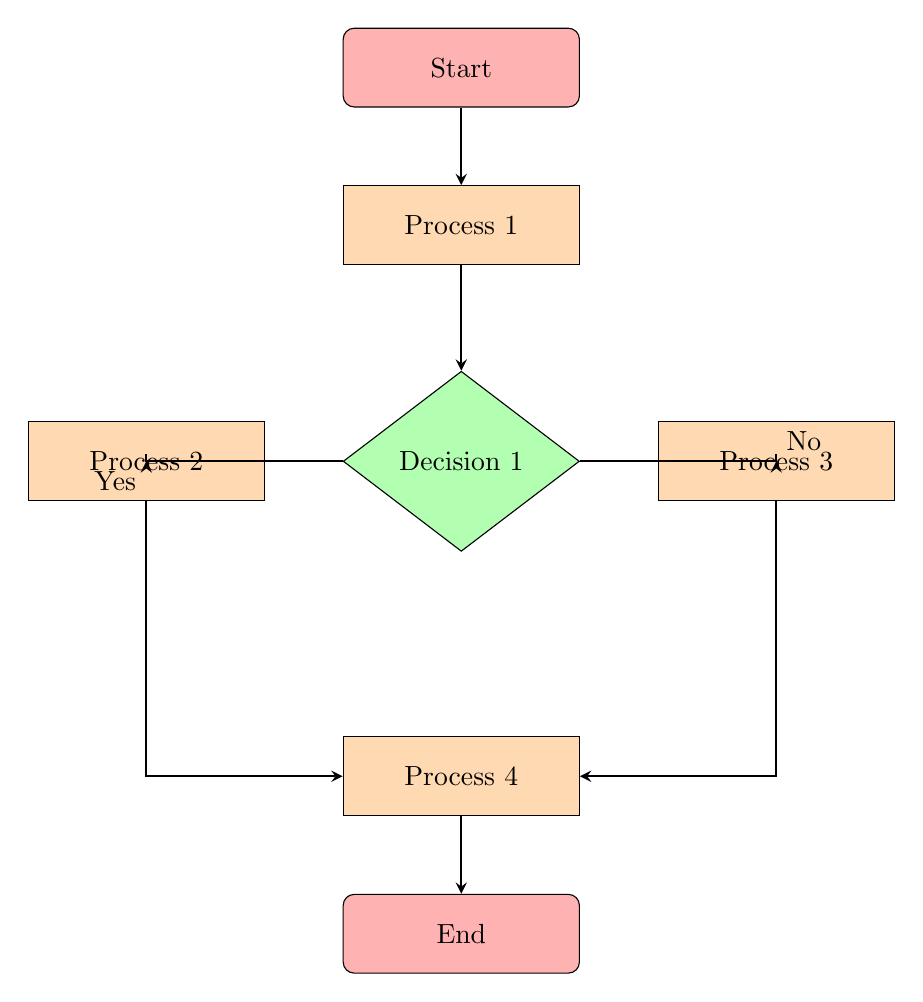
\begin{tikzpicture}[node distance=2cm]

\node (start) [startstop] {Start};
\node (process1) [process, below of=start] {Process 1};
\node (decision1) [decision, below of=process1, yshift=-1cm] {Decision 1};
\node (process2) [process, left of=decision1, xshift=-2cm] {Process 2};
\node (process3) [process, right of=decision1, xshift=2cm] {Process 3};
\node (process4) [process, below of=decision1, yshift=-2cm] {Process 4};
\node (end) [startstop, below of=process4] {End};

% Arrows
\draw [arrow] (start) -- (process1);
\draw [arrow] (process1) -- (decision1);
\draw [arrow] (decision1) -| node[anchor=north east] {Yes} (process2);
\draw [arrow] (decision1) -| node[anchor=south west] {No} (process3);
\draw [arrow] (process2) |- (process4);
\draw [arrow] (process3) |- (process4);
\draw [arrow] (process4) -- (end);

\end{tikzpicture}

\end{document}
